\documentclass[main.tex]{subfiles}\begin{document}

\chapter{Evaluation}
\label{chap:eval}
In this chapter, the plane detection algorithms selected in Section~\ref{sec:pdaselection} are uniformly compared. 
We enter this chapter by outlining the protocol followed during this evaluation.
Afterwards, we present and analyse the results thereof.

\section{Protocol}
This work aims to determine which plane detection algorithm is the most suitable for an AR/VR systems in a realistic environment. For this decision, we compare the algorithms selected in Chapter~\ref{chap:Concept}. 
In Section~\ref{sec:datasets}, we established that the 2D-3D-S dataset is not entirely suitable for evaluating real-world applicability due to its static nature, i.e., non-incremental growth and having been recorded by a stationary 360° camera.  To mitigate this, we created the realistic FIN dataset. 
Since both datasets are fundamentally different, we will perform the experiments and the analysis separately and then compare the results.
All experiments are performed on an AMD Ryzen 7 5800H CPU with 16GB of RAM.
First, we present the metrics used for comparison, followed by an outline of the used configurations of parameters for each experiment.

\subsection{Metrics}
\label{subsec:metrics}
The following two paragraphs detail the metrics we use in this evaluation. We introduce our methodology of measuring accuracy, as well as the calculation times. 
Note that by using the term "time frame $t$" or "time step $t$", we refer to the state of the point cloud at a given time $t$.

\paragraph{Accuracy}
To quantify the accuracy of the plane detection algorithms, we use the detected planes and the created ground truth to calculate the three following
metrics: Precision, \textit{Recall}, and the F1-Score.
We calculate the \textit{Precision}, as this reports the percentage of correctly detected points within the planes an algorithm returned.
Similarly, we calculate the \textit{Recall} because it gives information about the percentage of correctly detected points in comparison to the number of
points that \textit{could} be detected.
Using these metrics separately is problematic as we cannot expect the distribution of "plane" to "non-plane" to be even.
The \textit{F1-Score} is the harmonic mean of the \textit{Precision} and the \textit{Recall} and therefore measures the balance between the \textit{Precision} and
\textit{Recall}. Intuitively, this means that an algorithm has to yield sufficient \textit{Precision} and \textit{Recall} results to score
a sufficient \textit{F1-Score}. The \textit{F1-Score}, thereby, is the primary metric for the quantitative comparison of algorithms in this work.
However, we report the \textit{Precision} and the \textit{Recall} for thorough analysis.
The procedure of calculation is taken from~\cite[Section~4]{Araújo_Oliveira_2020} and detailed in Section~\ref{sec:metrics}.
Note that we use the detected planes for the calculation, however, we are not using them directly as a measure of performance due to the subjective
nature of manual ground truth segmentation.

\paragraph{Time Measurements}
\label{par:time}
We are also interested in the \textit{real-time} applicability of an algorithm.
We introduce two definitions of \textit{real-time} in Section~\ref{sec:realtime}.
To reiterate, we consider an algorithm to be \textit{totally real-time} ($RT_{tot}$) applicable if its total runtime is below $1s$.
Furthermore, we consider an algorithm to achieve \textit{Real-Time Plane Detection} ($RT_{calc}$) applicability if its plane detection and post-processing steps run faster than $1s.$

When recording a real environment, the point clouds likely grow incrementally with each map update.
Therefore, the average calculation time alone is of limited significance, as we assume the calculation times to grow with the cloud size.
Based on this assumption, it is necessary to analyze the relationship between the point cloud size and the calculation time in addition to average values.
Note that we refer to a point cloud's size by its number of contained points in the remainder of this chapter.

Following the separation of algorithms into phases (see Paragraph~\ref{par:prepostalgos}), we divide the calculation time into the pre-processing time $t_{pre}$,
the time spent during plane detection $t_{calc}$, and the duration of post-processing steps $t_{post}$.
This separation enables an in-depth analysis of both average results and the results over time.
Since we have two definitions of \textit{real-time}, we introduce two metrics of calculation time:

\begin{enumerate}
    \item The sum of $t_{calc}$ and $t_{post}$ allows us to determine whether an algorithm is \textit{Real-Time Plane Detection} applicable, \textit{and}
    \item to determine whether an algorithm is \textit{totally real-time} applicable, we consider the total computation time
          $t_{tot}$, which is the sum of the individual times (see Eq.~\ref{eq:tottime})
\end{enumerate}


\begin{equation}
    \label{eq:tottime}
    t_{tot} = t_{pre} + t_{calc} + t_{post}
\end{equation}

\subsection{Parameterization of Algorithms}
Because the datasets inherit different amounts of noise, it is necessary to modify the algorithms accordingly.
We thereby modify the algorithms' parameterization to achieve more noise robustness.
In the following, the parameterizations of the algorithms with respect to the two experiments are outlined.
Therein, we refer to the parameterization of the 2D-3D-S experiment as the default configuration.
Furthermore, we determine an appropriate parameterization for the FIN dataset through
empirical experiments. These experiments include multiple tests of different combinations of values on all scenes of the FIN dataset,
the ranges of which are specified in the respective paragraph of each algorithm.


\subsubsection{RSPD}
\begin{table}[H]
    \centering
    \caption[RSPD Parameterization]{Parameter configuration of RSPD used for the experiments.}
    \begin{tabular}{ccccccc}
        \toprule
        Experiment & $l_O$ & $\varepsilon$ & MOR  & $k$ & MND & MDP   \\ \hline
        2D-3D-S    & 10    & 30            & 25\% & 30  & 60° & 0.258 \\
        FIN        & 10    & 30            & 25\% & 30  & 60° & 0.258 \\
        \bottomrule
    \end{tabular}%
    \label{tab:rspd-param}
\end{table}

\paragraph{2D-3D-S}
We use the parameters of the provided implementation\footnote{\href{https://github.com/abnerrjo/PlaneDetection}{https://github.com/abnerrjo/PlaneDetection}} for the 2D-3D-S experiment. These parameters include the maximum octree level $l_O$,
the minimum number of samples per leaf node $\varepsilon$, the Maximum Outlier Ratio $MOR$ per plane, the size of the nearest neighborhood $k$,
the Maximum Normal Deviation $MND$, and the Maximum Distance to Plane $MDP$. Note that while $k=50$ is used in the respective paper~\cite[Section~3.3]{Araújo_Oliveira_2020},
$k=30$ is used in the official implementation. We adopted the latter because, in our experience, it produces sufficient results while reducing the pre-processing time.

\paragraph{FIN}
Multiple experiments with different values had been conducted. The individual ranges are $l_O \in [8,12], \varepsilon \in [15, 150], MOR \in [15, 40], k \in [30, 90], MND \in [50°, 70°]$, and $MDP \in [0.15, 0.4]$.
Through these experiments, we were not able to find a configuration that yields considerably better results than the default
parameterization. Therefore, no parameter modifications for the FIN dataset are made.


\subsubsection{OPS}

\begin{table}[H]
    \centering
    \caption[OPS Parameterization]{Parameter configuration of OPS used for the experiments.}
    \begin{tabular}{cccccc}
        \toprule
        Experiment & $\alpha_s$ & $KNN$       & $\theta_{h}$  & $\theta_{N}$ & $p$  \\ \hline
        2D-3D-S    & 3\%        & 30          & 0.05          & 100          & 0.99 \\
        FIN        & 3\%        & \textbf{90} & \textbf{0.35} & 100          & 0.99 \\
        \bottomrule
    \end{tabular}%
    \label{tab:ops-param}
\end{table}

\paragraph{2D-3D-S}
The parameter configuration used for the 2D-3D-S experiment is shown in the first row of Table~\ref{tab:ops-param}.
Like the parameterization of RSPD, we took this configuration from the provided implementation\footnote{\href{https://github.com/victor-amblard/OrientedPointSampling}{https://github.com/victor-amblard/OrientedPointSampling}}.
We use a sampling rate $\alpha_s$ of 3\% and a neighborhood size $KNN$ of 30 for the estimation of normal vectors.
Additionally, we use a distance threshold $\theta_h$ of 0.05(m).
Furthermore, we set the inlier threshold $\theta_N$ to 100 and the probability for adaptively determining RANSAC iterations
$p$ to $0.99$, as proposed in~\cite[Section~4A]{https://doi.org/10.48550/arxiv.1905.02553}.

\paragraph{FIN}
We ran experiments on the FIN dataset with different parameter values in the respective ranges:
$\alpha\in[0.3\%, 6\%]$, $KNN\in[30, 150]$, $\theta_h\in[0.05, 0.5]$, $\theta_N\in[50, 1000]$, and $p\in[0.90, 1.0]$.
We choose the configuration, that shows a balance between speed and accuracy, namely the following.
We increase $KNN$ to 90, as larger neighborhood sizes increase the accuracy of normal estimation and,
consequently, the overall accuracy of a method.
Furthermore, we increase the tolerated plane thickness $\theta_h$ because an increase in sensor noise ultimately thickens the recorded planes.
Both modifications are highlighted in bold in the second row of Table~\ref{tab:ops-param}.

\subsubsection{3D-KHT}
\begin{table}[H]
    \centering
    \caption[3D-KHT Parameterization]{Parameter configuration of 3D-KHT used for the experiments.}
    \begin{tabular}{cccccccc}
        \toprule
        Experiment & $\phi_{num}$ & $\rho_{num}$ & $s_{level}$ & $s_{ps}$ & $s_\alpha$ & $s_\beta$ \\ \hline
        2D-3D-S    & 30           & 200          & 2           & 0.002    & 18         & 6         \\
        FIN        & 30           & \textbf{100} & 2           & 0.002    & \textbf{8} & 6         \\
        \bottomrule
    \end{tabular}%
    \label{tab:3dkht-param}
\end{table}

\paragraph{2D-3D-S}
The parameter configuration is shown in Table~\ref{tab:3dkht-param}. We use an accumulator discretization of 30 and 200 for $\phi$ and $\rho$, respectively.
Starting to check for planarity at an octree level $s_{level}$ of 2 seems to yield the best results.
\citeauthor{LimbergerOliveira2015HT3D}~\cite{LimbergerOliveira2015HT3D} propose
a minimum of 30 samples per cluster $s_{ps}$, however, we use $0.2\%$ of the total point cloud due to the wide ranges of point cloud sizes in the dataset (see Subsection~\ref{subsec:bg-stanford}).
Lastly, we set the plane isotropy tolerance $s_\beta$ to 6, as proposed in~\cite[Section~3.1]{LimbergerOliveira2015HT3D}.
In contrast, using a plane thickness tolerance $s_\alpha$ value of 18 seemed to yield better results than the proposed 25.
This was determined by a small set of experiments with $s_\alpha$ values ranging between 15 and 33.

\paragraph{FIN}
For the FIN experiment, we modify the values of $\rho_{num}$, and $s_\alpha$ to accommodate for the higher levels of noise.
These values are obtained by performing tests with different parameterizations. Precisely, we used the following parameter ranges
combinations of values therein:
$\phi_{num} \in [20, 100]$, $\rho_{num} \in [50, 600]$, $s_{level}\in[1, 5]$, $\theta_N \in [50, 1000]$, $s_\alpha \in [5, 23]$, and $s_\beta \in [4, 8]$.
Reducing $\rho_{num}$ should decrease the accuracy, however, it seems to yield better results in a high-noise environment like the FIN dataset.
We decrease $s_\alpha$ to allow for slightly thicker, e.g. noisier, planes to be detected.
The modification of parameters is highlighted in bold in Table~\ref{tab:3dkht-param}.


\subsubsection{OBRG}
\begin{table}[H]
    \centering
    \caption[OBRG Parameterization]{Parameter configuration of OBRG used for the experiments.}
    \begin{tabular}{ccccccc}
        \toprule
        Experiment & $l_{max}$ & $\theta_{res}$ & $\theta_{d}$ & $\theta_{ang}$ & $\theta_M$ & $\theta_p$    \\ \hline
        2D-3D-S    & 5         & 0.08           & 0.08         & 0.18           & 5000       & 90\%          \\
        FIN        & 5         & \textbf{0.22}  & \textbf{0.2} & \textbf{0.2}   & 5000       & \textbf{70\%} \\
        \bottomrule
    \end{tabular}
    \label{tab:obrg-param}
\end{table}


\paragraph{2D-3D-S}
The used configurations for the experiments are shown in Table~\ref{tab:obrg-param}.
The parameterization was determined during the implementation process and showed a reasonable compromise between
efficiency and accuracy. 
We considered the reported parameterizations in~\cite[Tables~1,4,7]{Vo_Truong-Hong_Laefer_Bertolotto_2015}. However, since the authors used three large outdoor scenes for their evaluation, they would likely not be optimal for smaller, indoor scenes. We confirmed this assumption based on a small set of empiric experiments with scenes from the 2D-3D-S dataset, wherein we compared the results for the reported parameterization and the one we determined.
Due to the low level of noise, we assign a very small tolerance to the residual threshold $\theta_{res}$ and the distance threshold $\theta_d$.
Additionally, we assign a high planarity threshold value of $\theta_p = 90\%$.

\paragraph{FIN}
We performed tests with different parameterizations, individually ranging as follows.
$l_{max} \in [4\%, 7\%]$, $\theta_{res} \in [0.05, 0.3]$, $\theta_d \in [0.05, 0.3]$, $\theta_{ang}\in[0.13, 0.3], \theta_M \in [200, 6000]$,
and $\theta_p\in[70, 90]$.
Due to higher levels of noise, and thus, thicker walls, we increase $\theta_{res}$, $\theta_d$, and the angular divergence threshold $\theta_{ang}$.
According to~\cite[Section~3.4]{Vo_Truong-Hong_Laefer_Bertolotto_2015},
the planarity threshold $\theta_p$ should be chosen between 70\% and 90\% depending on the noise level. As the expected noise level of the
FIN dataset is much higher than the noise of the 2D-3D-S dataset, we reduce this threshold to 70\%.
The used parameters for the FIN experiment are summarized in the second row of Table~\ref{tab:obrg-param}.


\section{Results}
This section deals with the results of the experiments.
The individual results of both experiments are presented and analyzed. Lastly, the results are compared.


\subsection{2D-3D-S}

We ran RSPD, OPS, 3D-KHT, and OBRG on 139 scenes of the 2D-3D-S dataset. Subsequently, for each scene, the \textit{Precision, Recall,} and
the \textit{F1-Score} of each algorithm were calculated. The computation times were measured and divided into pre-processing $t_{pre}$, plane detection $t_{calc}$,
and post-processing $t_{post}$. Table~\ref{tab:res-3d2ds-total} shows the average of the computed results for each algorithm.
The rightmost column gives the total computation time $t_{tot}$. The largest values of the accuracy and the smallest average
values of the times are indicated in bold. It is to be noted that no lowest value of $t_{post}$ is indicated since RSPD and 3D-KHT
have no post-processing steps and, therefore, "per default" spend less time in this step.

\begin{table}[H]
    \centering
    \caption[Average 2D-3D-S Results]{Average results of each algorithm over the 2D-3D-S dataset. The right half of the inner columns shows the average time spent in
        pre-processing ($t_{pre}$), the average time spent in the plane detection ($t_{calc}$), and the average time spent in post-processing steps ($t_{post}$).
        The rightmost column shows the average total calculation time $t_{tot}$.
        Note that the absence of post-processing steps is denoted as "/". All times are measured in seconds.}
    \resizebox{\textwidth}{!}{%

        \begin{tabular}{c|ccc|ccc|c}
            \toprule
            \textbf{Algorithm} & \textbf{Precision} & \textbf{Recall}  & \textbf{F1-Score} & $\mathbf{t_{pre}}$ & $\mathbf{t_{calc}}$ & $\mathbf{t_{post}}$ & $\mathbf{t_{tot}}$ \\ \hline
            RSPD               & 84.80\%            & \textbf{89.79\%} & \textbf{86.84\%}  & 62.65              & 1.04                & /                   & 63.69              \\
            OPS                & \textbf{88.98\%}   & 70.45\%          & 77.68\%           & 13.12              & 10.97               & 1.01                & 25.10              \\
            3DKHT              & 71.40\%            & 78.32\%          & 75.19\%           & \textbf{0.71}      & \textbf{1.03}       & /                   & \textbf{1.74}      \\
            OBRG               & 81.38\%            & 66.77\%          & 71.00\%           & 28.07              & 34.29               & 2.61                & 62.97              \\
            \bottomrule
        \end{tabular}
    }
    \label{tab:res-3d2ds-total}
\end{table}

\paragraph{Accuracy}
RSPD has the overall highest accuracy with a \textit{Precision} of ${\sim}85\%$, a \textit{Recall} of ${\sim}90\%$, and an \textit{F1-Score} of ${\sim}87\%$.
OPS supersedes RSPD with a \textit{Precision} value of ${\sim}89\%$ but scores significantly lower \textit{Recall} and \textit{F1-Score} values.
3D-KHT yields \textit{Precision}, \textit{Recall} and \textit{F1-Score} results in the range of ${\sim}71\%$ and ${\sim}79\%$.
OBRG has a high \textit{Precision} value of ${\sim}81\%$, however its \textit{Recall} and \textit{F1-Score} values are the lowest out of all algorithms
with ${\sim}67\%$ and ${\sim}71\%$, respectively.

\paragraph{Average Time }
\label{par:2D-3D-S-time}
With an average of $0.71s$ spent in pre-processing, and an average of $1.03s$ spent in plane detection,
3D-KHT only needs an average total of $1.74s$ to process an entire point cloud and thereby achieves the lowest calculation times.
RSPD is the only algorithm that scores similar $t_{calc}$ values, with an
average of $1.04s$. However, RSPD's time spent in pre-processing is the highest among the algorithms.
With an average $t_{tot}$ of ${\sim}25s$ and ${\sim}63s$, OPS and OBRG, respectively, run dramatically slower than the other two algorithms.
According to these values, no algorithm achieves \textit{Total Real-time} applicability. RSPD and 3D-KHT are very close
to falling under the threshold of $1s$ for \textit{Real-Time Plane Detection} applicability, exceeding it by only $0.4s$ and $0.3s$, respectively


\paragraph{Relationship of Time and Size}
For each scene of the 2D-3D-S dataset, the pairs of processing times and point cloud file sizes are presented in Figure~\ref{fig:sizetimestanford}.

% \begin{figure}[H]
%     \centering
%     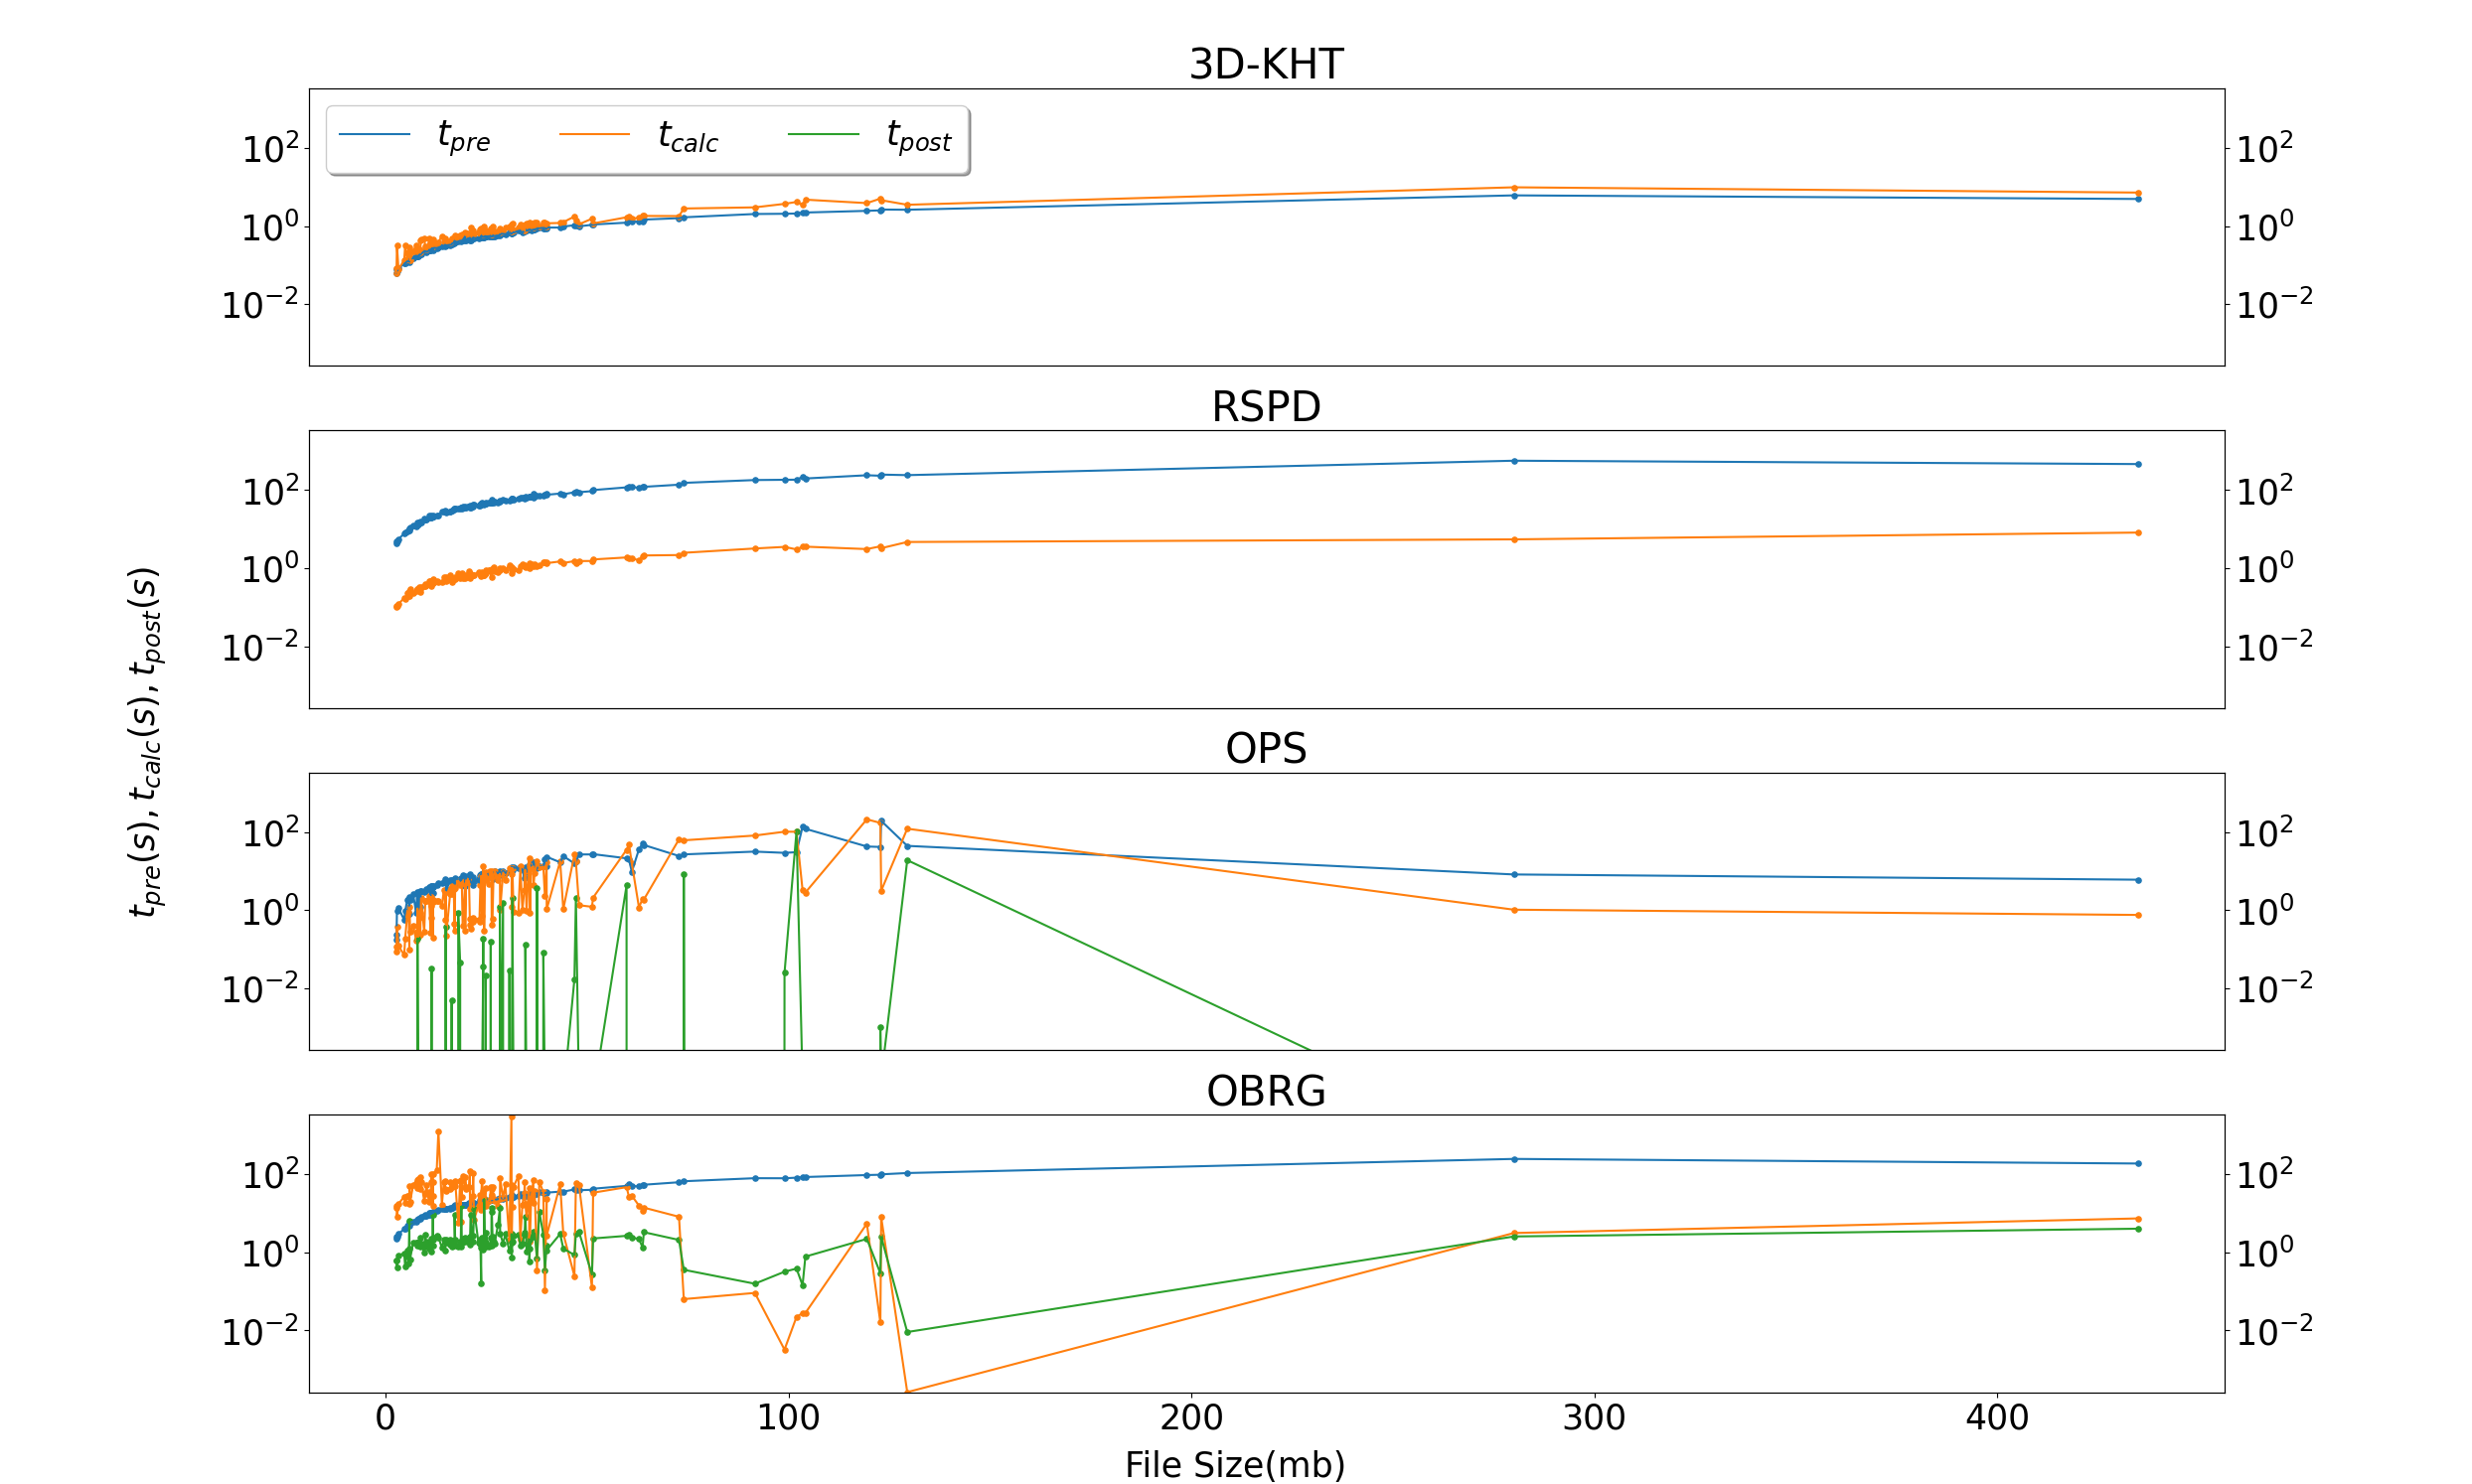
\includegraphics[width=\textwidth]{images/SDsizetime.png}
%     \caption[Time per Cloud size 2D-3D-S]{Time spent in pre-processing $t_{pre}$, plane detection $t_{calc}$,
%         and post-processing $t_{post}$ per point cloud file size of the 2D-3D-S dataset. Note that both y-axes are
%         scaled logarithmically to the base of ten.}
%     \label{fig:sizetimestanford}
% \end{figure}
\begin{figure}[]
    \centering
    \def\svgwidth{0.84\textwidth}
    \input{images/stanfordpdf.pdf_tex}
    \caption[Time Results 2D-3D-S]{The time spent in pre-processing $t_{pre}$, plane detection $t_{calc}$,
        post-processing $t_{post}$, and the total calculation time $t_{tot}$ per point cloud size of the 2D-3D-S dataset.
        Note that the y-axis is scaled logarithmically to the base of ten.}
    \label{fig:sizetimestanford}
\end{figure}
The computation times of 3D-KHT do not seem to strongly relate to the size of the point cloud.
Both the duration of the pre-processing and the duration of the plane detection initially grow linearly
but do not show a large growth even with large jumps in point cloud size.
The difference in calculation times between ${\sim}7\cdot10^6$ and ${\sim}9\cdot10^6$ is hardly noticeable considering .

The computation times of RPSD show a similar relation, with the difference that the pre-processing of RSPD takes significantly longer.
As with 3D-KHT, the duration of plane detection seems to have an upper limit.

In general, the pre-processing time of OPS has a linear growth depending on the size of the point cloud.
The duration of plane detection also shows a linear relationship, with the difference that there is a certain level
of fluctuation. The post-processing times are negligible for the most part, given the small number of values above $0$.
The irregularity of the spikes gives reason to assume that it primarily depends on the structure of the recorded
environment rather than size alone.

The duration of the pre-processing of OBRG also shows a linear relationship with respect to the point cloud size.
The average high $t_{pre}$ values from Table~\ref{tab:res-3d2ds-total} are also reflected here since most values are in the range of
$10s-100s$,
even for smaller cloud sizes at ${\sim}1\cdot10^6$.
The $t_{calc}$ values of OBRG do not appear to be dependent on the size of the point cloud, as the computation
times tend to decrease with growing point clouds. A possible reason could be the fixed value of the octree levels $l_{max}$.
As this parameter is vital for the calculations in all phases, all calculation times of OBRG are likely to show improvement
upon applying a parameter optimization of $l_{max}$ based on the dataset.
From our experience, the mid-sized scenes in the 2D-3D-S dataset are often long and narrow hallways. Assuming an inappropriate
octree depth parameter, the subdivision could effectively split the hallway, returning a set of chunks that are in no
way to be considered planar. This would consequently lead to an early termination due to failed thresholds, thus reducing
the calculation times (and most likely yielding low accuracy).

\paragraph{Summary 2D-3D-S Experiment}
\label{par:sumsdexp}
With an average of ${\sim}89\%$, OPS has the highest value in \textit{Precision}, while RSPD achieves the highest \textit{Recall}
and \textit{F1-Score} with ${\sim}90\%$ and ${\sim}87\%$, respectively.
3D-KHT has the lowest total computation time $t_{tot}$ with an average of $1.74s$. With ${>}60s$,
RSPD and OBRG have the largest $t_{tot}$ values among the algorithms, with $t_{pre}$ accounting for
the majority for RSPD.


Figure~\ref{fig:sizetimestanford} shows that the runtimes of 3D-KHT are the smallest. RSPD also has low $t_{calc}$ values
but consistently spends the longest time in pre-processing.
Moreover, the pre-processing times of all algorithms seem to be generally dependent on the size of the point cloud.
The plane detection runtimes of OPS and OBRG fluctuate. However, OPS fluctuates less than OBRG.
The post-processing runtimes of OPS are negligible overall. The $t_{post}$ values of OBRG are stable at $2.61s$ on average,
except for medium cloud sizes, see Table~\ref{tab:res-3d2ds-total}.

Adhering strictly to our definitions of \textit{real-time}, no algorithm achieves \textit{real-time} applicability in this experiment.
However, we might consider RSPD and 3D-KHT to be \textit{Real-Time Plane Detection} applicable since
the point cloud sizes vary greatly, and the average duration of their plane detection phase is only
$0.03s-0.04s$ greater than the $1s$ threshold.
Furthermore, as Figure~\ref{fig:sizetimestanford} suggests, RSPD and 3D-KHT are
\textit{Real-Time Plane Detection} applicable for point clouds with ${\lesssim}1\cdot10^6$ points.

\subsection{FIN}
Each of the total 708 time frames of the FIN data set was processed by each algorithm.
Subsequently, we evaluated each time frame separately, i.e., by calculating the \textit{Precision, the Recall,} and the \textit{F1-Score} .
Additionally, we measured the computation times of each time frame for all algorithms, again divided into pre-processing $t_{pre}$,
plane detection $t_{calc}$, and post-processing $t_{post}$.

The average results over all time steps of all scenes of the FIN experiment are presented in Table~\ref{tab:res-fin-total}.
The highest values are written in bold for \textit{Precision, Recall,} and the \textit{F1-Score}, as are the lowest times of each calculation step and the
total time.


\begin{table}[]
    \centering
    \caption[Average FIN Results]{Average Results of the FIN experiment. Shown are the average values of all scenes and time frames, sorted by
        algorithm. The right half of the columns shows the average time spent in pre-processing ($t_{pre}$), the average time spent in the plane
        detection itself ($t_{calc}$), and the average time spent in post-processing steps ($t_{post}$).
        The rightmost column shows the average total calculation time $s_{tot}$.
        Note that the absence of post-processing steps is denoted as "/".
        All times are measured in seconds.}
    \resizebox{\textwidth}{!}{%
        \begin{tabular}{c|ccc|ccc|c}
            \toprule
            \textbf{Algorithm} & \textbf{Precision} & \textbf{Recall}  & \textbf{F1-Score} & $\mathbf{t_{pre}}$ & $\mathbf{t_{calc}}$ & $\mathbf{t_{post}}$ & $\mathbf{t_{tot}}$ \\ \hline
            RSPD               & 57.30\%            & \textbf{60.75\%} & \textbf{58.70\%}  & 14.36              & \textbf{0.19}       & /                   & 14.55              \\
            OPS                & \textbf{69.38\%}   & 29.23\%          & 39.43\%           & 4.61               & 0.89                & 0.13                & 5.63               \\
            3DKHT              & 49.76\%            & 44.40\%          & 46.48\%           & \textbf{0.14}      & 0.29                & /                   & \textbf{0.43}      \\
            OBRG               & 49.23\%            & 27.42\%          & 33.94\%           & 6.03               & 14.70               & 0.35                & 21.08              \\
            \bottomrule
        \end{tabular}
    }
    \label{tab:res-fin-total}
\end{table}

\paragraph{Accuracy}
OPS has the highest average \textit{Precision} of the algorithms, with almost 70\%. RSPD achieves the highest values
for \textit{Recall} and the \textit{F1-Score} with ${\sim}61\%$ and ${\sim}59\%$, respectively.
3D-KHT and OBRG achieve a similar \textit{Precision}, but for \textit{Recall} and \textit{F1-Score}, however, 3D-KHT has
higher values than OBRG by approx. 13\% and approx. 17\%, respectively.
RSPD thus achieves the highest overall accuracy, while OBRG achieves the overall lowest.


\paragraph{Average Time}
With almost $15s$, RSPD spends the most time in pre-processing among the algorithms. In contrast, RSPD has the shortest time spent
during plane detection, with an average of $0.19s$. Overall, 3D-KHT needs the shortest time for the complete computation $t_{tot}$
of a time step with an average of $0.43s$. OPS achieves comparatively average total calculation time with ${\sim}6s$, and OBRG
takes the longest overall to compute a time step with more than $20s$.

RSPD and 3D-KHT achieve \textit{Real-Time Plane Detection} applicability. Additionally, 3D-KHT also achieves \textit{Total Real-time} applicability,
with an average total time of $0.43s$. OPS can almost be considered to be in $RT_{calc}$ with a subtotal
calculation time of $1.02s$, thereby taking $0.02s$ too long.
With an average pre-processing time of ${\sim}6s$ and an average of ${\sim}15s$ spent in plane detection, OBRG qualifies for
neither of the introduced definitions of \textit{real-time}.


\paragraph{Relationship of Time and Size}
As mentioned before in Paragraph~\ref{par:time}, we are interested in the relationship between the size of the point cloud and the corresponding calculation time.
In Figure~\ref{fig:dynaudi}, we compare the processing times of each time step to the number of points in the
\textit{auditorium} scene of the FIN data set.

\begin{figure}[H]
    \centering
    \def\svgwidth{0.7\textwidth}
    % \input{images/dynaudi.pdf_tex}
    \input{images/dynaudi_crop.pdf_tex}
    \caption[Time Results Auditorium Scene]{Time spent in pre-processing $t_{pre}$, plane detection $t_{calc}$, post-processing
    $t_{post}$, and total calculation time $t_{tot}$ of the \textit{auditorium} scene, and point cloud size of each time frame.
    Note that both y-axes are scaled logarithmically to the base of ten. \textit{Time Frames} are defined in Subsection~\ref{subsec:metrics}.}
    \label{fig:dynaudi}
\end{figure}
\clearpage
Note that we created similar graphs for the other scenes of the FIN dataset.
However, they do not introduce new information into the argumentation and are presented in Appendix~\ref{app:fin} for completeness
and spatial reasons.
We consider the \textit{auditorium} scene as the most representative because it contains the longest recording, and thus contains the most data.

The pre-processing times of RSPD and OBRG are noticeably proportional to the point cloud size.
In contrast, for OPS and 3D-KHT, the pre-processing times seem to correlate with the plane detection times since
both show similar spikes. The plane detection steps of OPS and 3D-KHT do not seem to depend on the point cloud size,
as both seem to be limited by an upper bound, ${\sim}1s$ for 3D-KHT and ${\sim}6s$ for OPS. The pre-processing and plane detection times of OBRG grow rapidly in the
beginning but afterward, show a linear growth in relation to the cloud size. The post-processing times of OPS fluctuate
between 0 and the duration of plane detection. After the spike in the beginning, the $t_{post}$ values of OBRG seem to be
consistent.

The apparent upper bound of ${\sim}1s$ in the calculation times qualifies 3D-KHT for
\textit{Total Real-time} applicability.
We consider RSPD \textit{Real-Time Plane Detection} applicable, as the duration of the
plane detection step consistently stays under $1s$.

\paragraph{Summary FIN Experiment}
\label{par:sumfinexp}
OPS has the highest average \textit{Precision}, and RSPD has the largest percentages of \textit{Recall} and the \textit{F1-Score} .
Additionally, RSPD has the lowest $t_{calc}$ value among the algorithms,
with an average of $0.19s$ per time frame. In contrast, RSPD has the longest pre-processing time with $14.36s$ on average.
The algorithm with the shortest pre-processing and the shortest total time is 3D-KHT with $t_{pre}=0.14s$ and $t_{tot}=0.43s$,
respectively.


In general, the calculation times of RSPD and OBRG seem to depend on the point cloud size.
However, the time RPSD spends in pre-processing is significantly higher than in its plane detection step.
In contrast, the pre-processing and plane detection times of OBRG seem to converge at the end.
The calculation times of OPS and 3D-KHT seem to be independent of the point cloud size and consistently stay under an upper bound.
However, 3D-KHT has a smaller upper bound than OPS.

The development over time supports the average calculation times of 3D-KHT, as the calculation
seems independent of the cloud size. Thereby, we determine 3D-KHT to be \textit{Total Real-time}
applicable.
Furthermore, RSPD achieves \textit{Real-Time Plane Detection} applicability in the FIN experiment, as the
plane detection step takes $<1s$ for all time frames.
Lastly, the average subtotal calculation time of OPS is slightly longer than $1s$. However, given
the apparent upper bound and considerable fluctuations, we cautiously consider OPS to be
\textit{Real-Time Plane Detection} applicable in the FIN experiment.

\subsection{Comparison}
When comparing Table~\ref{tab:res-3d2ds-total} and Table~\ref{tab:res-fin-total}, a pattern emerges:
OPS has the highest \textit{Precision} value, RSPD yields the highest \textit{Recall} and \textit{F1-Score}, and 3D-KHT has the lowest
average total processing time.

Observing Figure~\ref{fig:dynaudi} and Figure~\ref{fig:sizetimestanford}, common features are noticeable:
The curve shape of RSPD is very similar for both experiments, linearly dependent on the point cloud size, and the
$t_{pre}$ accounts for $99\%$ of the total calculation time $t_{tot}$.
In both experiments, the post-processing time of OPS fluctuates.
The post-processing of OBRG seems to be oriented around a given value, however, this value differs
between the experiments (${\sim}0.3s$ for the FIN experiment and ${\sim}3s$ for the 2D-3D-S experiment).
3D-KHT scores very low processing times in both experiments.

However, there are also notable differences.
Whereas the calculation times of 3D-KHT seem to be proportional to the point cloud size in the 2D-3D-S experiment, they show no such
relation during the FIN experiment. It is worth noting that the cloud sizes widely differ between the experiments, as the
maximum size of the FIN experiment (${\sim}0.75\cdot10^6$) is very small, compared to largest scene of the 2D-3D-S dataset (${\sim}9\cdot10^6$).
Nonetheless, since Figure~\ref{fig:sizetimestanford} portrays a proportionality, even for smaller clouds, the reason for
different curves is likely the difference of parameterization.

In Paragraph~\ref{par:sumsdexp}, we report that no algorithm is \textit{real-time} applicable. We state, that
RSPD and 3D-KHT can be considered \textit{Real-Time Plane Detection} applicable since the cloud sizes vary and
the difference between their average $t_{calc}$ times and the threshold of $1s$ is very small.
In Paragraph~\ref{par:sumfinexp}, we consider 3D-KHT \textit{totally real-time} applicable due to the observed
upper bound in calculation time in combination with a low average $t_{tot}$ value of $0.43s$. Additionally,
we consider $RSPD \in RT_{calc}$ because RSPD takes consistently less than $1s$ during the plane detection step.
The results of neither experiment show a \textit{real-time} applicability of OBRG.


\section{Summary}
OBRG achieves neither the highest nor lowest values in any experiment.
OPS has the highest \textit{Precision} in both experiments.
Due to \textit{Recall} and the \textit{F1-Score}, RSPD has the highest overall accuracy in both experiments.
The pre-processing of RSPD takes the longest time of all algorithms. In contrast, RSPD has the smallest average $t_{calc}$
value in the FIN experiment. 3D-KHT has the lowest total computation time in both experiments, and in the 2D-3D-S experiment,
it outperforms the plane detection time of RSPD.

3D-KHT is \textit{Real-Time Plane Detection} applicable in the 2D-3D-S experiment and \textit{totally real-time} applicable
in the FIN experiment.
RSPD achieves \textit{Real-Time Plane Detection} applicable in both experiments.
We consider OPS to be \textit{Real-Time Plane Detection} applicable.
These achieved \textit{real-time} applicabilities are summarized in Table~\ref{tab:algo-rt}.
% NOTE 3DKHT kann keine löcher oder non-rectangular ebenen basteln!

\begin{table}[H]
    \centering
    \caption[Real-Time Applicabilities of Selected Algorithms]{Real-time applicabilities of the selected plane detection algorithms given the results from both experiments.
        Note that $RT_{tot}$ implies $RT_{calc}$. "/" denotes no \textit{real-time} applicability.
        "*" denotes that the given \textit{real-time} applicability is coupled with a restriction. We refer to the text for details.}
    \begin{tabular}{ccccc}
        \toprule
        \textbf{Experiment} & \textbf{RSPD} & \textbf{OPS} & \textbf{3D-KHT}     & \textbf{OBRG} \\
        \midrule
        2D-3D-S             & $RT_{calc}$*  & /            & $RT_{calc}$*        & /             \\
        FIN                 & $RT_{calc}$   & $RT_{calc}$* & $\mathbf{RT_{tot}}$ & /             \\
        \bottomrule
    \end{tabular}
    \label{tab:algo-rt}
\end{table}

\end{document}